\newpage
\begin{slikaDesno}[0.83]{fig/tram.pdf}
    \PID 
На слици \ID.1 приказан је упрошћени модел 
електричног трамваја масе $m = 20\unit{t}$ који
се креће по равној прузи. Трамвај 
се напаја из мреже константног напона $V_{\rm S} = 
650\unit{V}$. Мотор трамваја се представља 
идеалним струјним генератором, струје 
$i_{\rm g} = i_{\rm g}(t)$, која се 
може контролисати. Претпоставити да се сва снага
коју мрежа предаје мотору, без губитака, претвара у механичку 
енергију посредством механичке силе. 
На трамвај делује и сила отпора ваздуха
дата изразом ${\bf F}_{\rm ov} = -b {\bf v}$, где је\linebreak 
\vspace*{-3mm}
\end{slikaDesno} 
$b = 150\unit{\dfrac{N}{km/h}}$ a 
$v = v(t)$ је брзина трамваја.
Посматрамо систем чији једини
улаз представља струја $i_{\rm g}$ а једини
излаз тренутна брзина $v$ трамваја. 
Ако је познато да се тај систем може представити 
као каскадна веза једног линеарног система 
чија је функција преноса $H(s)$ и једног 
нелинеарног система без меморије чија је 
статичка преносна карактеристика $f(u)$,
одредити једно решење за 
$H(s)$ и $f(u)$. Објаснити да ли 
је посматрани систем линеаран.
Скицирати временски дијаграм тренутне брзине 
трамваја ако је управљачка струја дата изразом
$i_{\rm g} = I_0 \operatorname{rect}
\left( \dfrac{t}{T} - 1 \right)$,
где су $I_0 = 250\unit{A}$ и $T = 20\unit{s}$,
а трамвај полази из мировања.
\vspace*{1mm}

\noindent
\textit{\underline{Помоћ.}} Снага механичке силе $F$ која 
делује на круто тело које се креће брзином $v$ 
равна је $P = Fv$. \\

\textsc{\underline{Решење}}: (а) Укупна механичка снага која делује на трамвај разлика је снаге 
коју улаже генератор и снаге губитака на отпор ваздуха, 
\begin{equation}
P_{\rm meh} = P_{\rm g} - P_{\rm ov}. \label{eq:\ID.1}
\end{equation}
Снагом генератора се управља индиректно помоћу управљачке
струје, $P_{\rm g} = V_{\rm S} i_{\rm g}$ док је снага губитака на рачун отпора ваздуха 
$P_{\rm ov } = F_{\rm ov} v = -bv^2$. Пошто се трамвај креће по равној прузи механички рад 
претвара се у кинетичку енергију па је
$P_{\rm meh} = \dfrac{\de W_{\rm k}}{\de t} = \dfrac{m}{2} \dfrac{\de (v^2)}{\de t}$. Заменом 
свих одређених снага у израз добија се диференцијална једначина \eqref{eq:\ID.1}:
\begin{equation}
    \dfrac{m}{2} \dfrac{\de (v^2)}{\de t} =
    V_{\rm S} i_{\rm g} - bv^2
\end{equation}
%
\begin{figure}[b!]
    \centering
    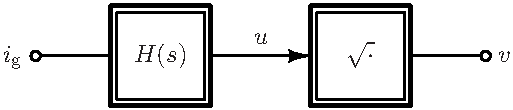
\includegraphics[scale=1]{fig/tram_diag.pdf}
    \caption{}
\end{figure}
%
Добијена диференцијална једначина по $v$ није линеарна, али се може приметити да је линеарна по $v^2$ што 
користимо увођењем одговарајуће смене $u = v^2$, чиме се добија диференцијална једначина  
на основу које се лако може наћи преносна функција $H(s) = \dfrac{U(s)}{I_{\rm g}(s)}$ \vspace*{1mm} као 
\begin{equation}
    \dfrac{m}{2} \dfrac{\de u}{\de t} =
    V_{\rm S} i_{\rm g} - bu \bigg|_{\mathcal L} \Rightarrow
    \dfrac{sm}{2} U(s) = V_S I_{\rm g}(s) - b U(s) \Rightarrow 
    H(s) = \dfrac{V_{\rm S}}{ \dfrac{m}{2} s + b }
\end{equation}
Одговарајућа смена се може третирати као нелинеарни систем без меморије, па је тако у целини 
дати систем представљен каскадном везом линеарног система функције преноса $H(s)$ и нелинеарног система
без меморије статичке преносне карактеристике $f(u) = \sqrt{u}$ као на слици \ID.2.

(б) Линеарност система проверава се испитивањем хомогености и адитивности. Систем је хомоген уколико, вреди 
$O\{kx(t)\} = kO\{x(t)\}$. Посматраћемо брзину у устаљеном стању, односно када је 
$\dfrac{\de v^2}{\de t} \to 0$, тада важи да је $V_{\rm S} i_{\rm g}(\infty) - bv(\infty)^2 \to 0$, односно 
$v(\infty) = \sqrt{\dfrac{V_{\rm S} i_{\rm g}(\infty)}{b}}$. На основу израза се види да је 
$v(\infty) \propto i_{\rm g}(\infty)$ па систем није хомоген, а самим тим ни линеаран. 
Нагласимо да у општем случају каскадна веза линеарног 
и нелинеарног система није линеаран систем, ипак, постоје практичне примене у којима се користе нелинеарни системи за изградњу система
који су у целини линеарни (нпр. транслинеарна кола у аналогној електроници).


\begin{figure}[b!]
    \centering
    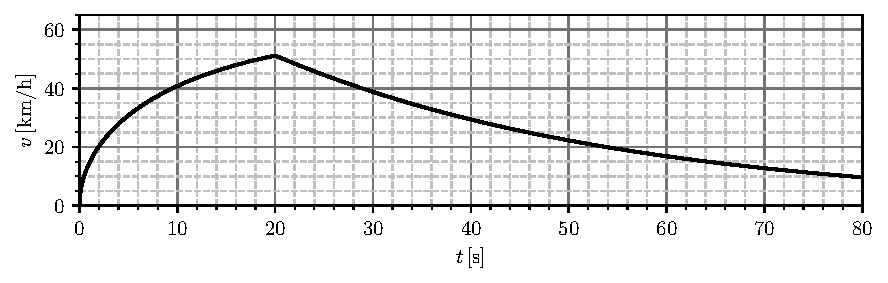
\includegraphics[scale=1]{fig/tram_plot.pdf}
    \caption{}
\end{figure}

    (в) Одзив на задату побуду одредићемо одређивањем међурешења $u(t)$. Побуда се може записати у облику 
    $i_{\rm g} = I_0 (u(t) - u(t - T))$. Тако да ће одзив бити 
    $u(t) = I_0 (g(t) - g(t - T))$, где је $g(t)$ одскочни одзив система $H(s)$, због његове линеарности. 
    Одскочни одзив одређујемо у комплексном домену, растављањем на парцијалне разломке
    \begin{align}
        G(s) = \underbrace{\dfrac{1}{s}}_{\LT{\uu(t)}} \cdot \underbrace{\dfrac{V_{\rm S}}{ \dfrac{m}{2} s + b } }_{H(s)}
        = \dfrac{A}{s} + \dfrac{B}{\dfrac{m}{2} s + b} 
        = 
        \begin{cases}
            A =  \dfrac{V_{\rm S}}{ \xcancel{s}\left( \dfrac{m}{2} s + b\right) } \bigg|_{s = 0} = \dfrac{V_{\rm S}}{b} \\
            B =  \dfrac{V_{\rm S}}{ {s} \,\, \xcancel{\left( \dfrac{m}{2} s + b\right) } } \bigg|_{s = -\frac{2b}{m}} = 
            -\dfrac{m V_{\rm S}}{2b}
        \end{cases}
    \end{align}
    Сређивањем добијеног израза добија се 
    $
    G(s) = \dfrac{V_{\rm s}}{b} \left( \dfrac{1}{s} - \dfrac{1}{s + \frac{2b}{m}} \right)$ \vspace*{1mm} 
    па се инверзном Лапласовом трансформацијом налази
    $g(t) = \mathcal{L}^{-1} \{ G(s) \} = \dfrac{V_{\rm S}}{b} \left(1 - \ee^{ -\frac{2b}{m} t } \right) \uu(t) $, 
    сређивањем се даље налази
    \begin{equation}
    u(t) = \dfrac{I_0 V_{\rm S}}{b} \Biggl(
        \left(1 - \ee^{ -\frac{2b}{m} t } \right) \uu(t) 
        -
        \left(1 - \ee^{ -\frac{2b}{m} (t - T)} \right) \uu(t - T),
    \Biggr)
    \end{equation}
    што се може расписати и као 
    \begin{eqnarray}
        u(t) = \dfrac{I_0 V_{\rm S}}{b} \cdot 
        \begin{cases}
            0 , & t < 0 \\
            1 - \ee^{-\frac{2b}{m}t} , & 0 < t < T \\
            ( \ee^{2bT/m} - 1) \ee^{-\frac{2b}{m}t} , & t > T 
        \end{cases}
    \end{eqnarray}
    па је израз за брзину са израчуатим константама: 
    \begin{eqnarray}
        v(t) \approx 62,5 \unit{\dfrac{km}{h}} \cdot 
        \sqrt{
        \begin{cases}
            0 , & t < 0 \\
            1 - \ee^{-t/18\unit{s}} , & 0 < t < T \\
            2,04\, \ee^{-t/18\unit{s}} , & t > T 
        \end{cases}
        }
    \end{eqnarray} 
    Добијени резултат приказан је на слици.




    
